\section{Results}
\label{sec:results}

\subsection{Reading is not writing}
\label{sec:headline}

Table~\ref{tab:cf-main} reports scores for every checkpoint on every dataset. Figure~\ref{fig:overview} shows every concept cell across the three grades. Both chest datasets follow the same pattern. On the calibration cohort, clinical concepts are readable in \cfChestReadable{} of \cfChestReadableN{} cells (\cfChestReadablePct\%): probe selectivity exceeds matched random-label controls by $0.1$--$0.3$ for most findings in most families. The models also answer on this cohort: \cfChestAnswerable{} of the \cfChestAnswerableN{} cells with a scored write matrix (\cfChestAnswerablePct\%) have a clean-answer AUROC lower bound above chance on the same 400 rows. Of these answerable cells, \cfReadAns{} are also readable. Yet only \cfChestOwned{} cells (\cfChestOwnedPct\%) are owned. In \cfChestCompetitor{} cells (\cfChestCompetitorPct\%), the verdict is \emph{stronger competitor}: a direction fitted for another finding moves the concept's answer more than the concept's own direction does. Readability and answerability do not suffice for writing: only \cfReadAnsOwned{} of the \cfReadAns{} readable and answerable cells are owned (\cfReadAnsOwnedPct\%), compared with \cfRestOwned{} of the remaining \cfRestN{} (\cfRestOwnedPct\%).

Table~\ref{tab:cf-contingency} groups chest cells by steering-reference status and clinical comparison verdict. To meet the steering reference, the concept's own write must raise its answer above both the 95th percentile of the random writes and the absolute sham. Of the \cfChestAnswerableN{} chest cells, \cfChestRefMet{} meet this reference. Among these \cfChestRefMet{} cells, \cfChestOwned{} are owned, \cfChestRefStrong{} have a stronger competitor, and \cfChestRefUnres{} are unresolved. The remaining \cfChestRefBelow{} cells fall below the steering reference and account for \cfChestBelowStrong{} of the \cfChestCompetitor{} stronger-competitor verdicts (\cfChestBelowStrongPct\%). In these cells, the concept's own write fails to clear the random and sham references. A direction fitted for another finding moves the concept's answer more. Readable and answerable cells show the same pattern. Of the \cfReadAns{} readable and answerable cells, \cfReadAnsRefMet{} meet the steering reference. Among these, \cfReadAnsOwned{} are owned, \cfReadAnsRefStrong{} have a stronger competitor, and \cfReadAnsRefUnres{} are unresolved. Of the \cfReadAnsCompetitor{} stronger-competitor verdicts for readable and answerable cells, \cfReadAnsBelowStrong{} occur in the \cfReadAnsRefBelow{} cells below the reference. On COCO, \cfCocoRefMet{} of \cfCocoOwnedN{} cells meet the steering reference. Of these, \cfCocoOwned{} are owned. Of the \cfCocoCompetitor{} stronger-competitor verdicts, \cfCocoBelowStrong{} occur below the reference.

\begin{table}[t]
\centering
\scriptsize
\setlength{\tabcolsep}{2pt}
\renewcommand{\arraystretch}{1.08}
% Morandi tints for the cf-transfer tables (muted, low saturation); darker = larger value
\definecolor{cfSage1}{HTML}{EEF1EA}
\definecolor{cfSage2}{HTML}{D9E1D2}
\definecolor{cfSage3}{HTML}{C1CDB8}
\definecolor{cfSage4}{HTML}{A6B79C}
\definecolor{cfSlate1}{HTML}{ECEFF2}
\definecolor{cfSlate2}{HTML}{D3DAE2}
\definecolor{cfSlate3}{HTML}{B7C3D0}
\definecolor{cfSlate4}{HTML}{98A8B9}
\definecolor{cfTerra1}{HTML}{F5ECE9}
\definecolor{cfTerra2}{HTML}{E9D3CC}
\definecolor{cfTerra3}{HTML}{DAB5AA}
\definecolor{cfTerra4}{HTML}{C9968A}
\definecolor{cfOat1}{HTML}{F4EFE6}
\definecolor{cfOat2}{HTML}{E8DDC8}
\definecolor{cfGrey}{HTML}{E4E1DC}

\caption{\textbf{Reading, answering, and writing per checkpoint.} Per dataset: mean probe selectivity (\textsc{Read}), clean-answer AUROC (\textsc{Ans}), and ownership (\textsc{Own}), superscripted with the graded concepts of six, then the owned share of clinical and COCO cells and their ratio. Grey marks an ineligible template (inel.), an incomplete write matrix (inc.); ``--'' is a block not run.}
\label{tab:cf-main}
\begin{tabular}{l@{\hspace{3pt}}ccc@{\hspace{4pt}}ccc@{\hspace{4pt}}ccc@{\hspace{4pt}}ccc}
\toprule
& \multicolumn{3}{c}{NIH ChestX-ray14} & \multicolumn{3}{c}{CheXpert Plus} & \multicolumn{3}{c}{COCO (control)} & \multicolumn{3}{c}{Owned share} \\
\cmidrule(lr){2-4}\cmidrule(lr){5-7}\cmidrule(lr){8-10}\cmidrule(lr){11-13}
Checkpoint & \textsc{Read} & \textsc{Ans} & \textsc{Own} & \textsc{Read} & \textsc{Ans} & \textsc{Own} & \textsc{Read} & \textsc{Ans} & \textsc{Own} & clin. & COCO & ratio \\
\midrule
Lingshu 32B & \cellcolor{cfSage2}0.08$^{3}$ & \cellcolor{cfSage3}0.78$^{6}$ & \cellcolor{cfTerra2}-0.02$^{2}$ & \cellcolor{cfSage4}0.20$^{4}$ & \cellcolor{cfSage3}0.87$^{5}$ & \cellcolor{cfSlate2}+0.04$^{5}$ & \cellcolor{cfSage1}0.03$^{1}$ & \cellcolor{cfSage4}0.95$^{5}$ & \cellcolor{cfSlate4}+0.28$^{6}$ & \cellcolor{cfSlate4}58\% & \cellcolor{cfSlate4}100\% & 58\% \\
CheXagent-2-3B & \cellcolor{cfSage3}0.13$^{5}$ & \cellcolor{cfSage3}0.86$^{6}$ & \cellcolor{cfSlate1}+0.00$^{2}$ & \cellcolor{cfSage4}0.21$^{5}$ & \cellcolor{cfSage4}0.95$^{5}$ & \cellcolor{cfSlate1}+0.01$^{4}$ & \cellcolor{cfSage3}0.13$^{4}$ & \cellcolor{cfSage3}0.81$^{5}$ & \cellcolor{cfSlate2}+0.03$^{2}$ & \cellcolor{cfSlate4}50\% & \cellcolor{cfSlate2}33\% & 150\% \\
Qwen2.5-VL-72B & \cellcolor{cfSage2}0.07$^{2}$ & \cellcolor{cfSage2}0.62$^{4}$ & \cellcolor{cfTerra2}-0.03$^{3}$ & \cellcolor{cfSage3}0.20$^{4}$ & \cellcolor{cfSage2}0.71$^{4}$ & \cellcolor{cfTerra2}-0.09$^{1}$ & \cellcolor{cfSage1}0.01$^{1}$ & \cellcolor{cfSage4}0.99$^{5}$ & \cellcolor{cfSlate4}+0.66$^{6}$ & \cellcolor{cfSlate3}33\% & \cellcolor{cfSlate4}100\% & 33\% \\
Lingshu 7B & \cellcolor{cfSage2}0.08$^{3}$ & \cellcolor{cfSage3}0.76$^{6}$ & \cellcolor{cfSlate2}+0.02$^{1}$ & \cellcolor{cfSage4}0.21$^{4}$ & \cellcolor{cfSage3}0.86$^{5}$ & \cellcolor{cfSlate2}+0.04$^{3}$ & \cellcolor{cfSage1}0.02$^{1}$ & \cellcolor{cfSage4}0.97$^{5}$ & \cellcolor{cfSlate4}+0.68$^{6}$ & \cellcolor{cfSlate3}33\% & \cellcolor{cfSlate4}100\% & 33\% \\
Qwen3-VL-4B & \cellcolor{cfSage2}0.08$^{3}$ & \cellcolor{cfSage2}0.71$^{6}$ & \cellcolor{cfTerra3}-0.11$^{0}$ & \cellcolor{cfSage4}0.20$^{4}$ & \cellcolor{cfSage2}0.74$^{4}$ & \cellcolor{cfTerra1}-0.01$^{2}$ & \cellcolor{cfSage1}0.04$^{4}$ & \cellcolor{cfSage4}0.99$^{5}$ & \cellcolor{cfSlate4}+0.34$^{6}$ & \cellcolor{cfSlate3}17\% & \cellcolor{cfSlate4}100\% & 17\% \\
Qwen3-VL-32B & \cellcolor{cfSage2}0.10$^{2}$ & \cellcolor{cfSage2}0.70$^{6}$ & \cellcolor{cfTerra2}-0.02$^{1}$ & \cellcolor{cfSage3}0.17$^{5}$ & \cellcolor{cfSage3}0.82$^{5}$ & \cellcolor{cfTerra2}-0.02$^{1}$ & \cellcolor{cfSage2}0.05$^{4}$ & \cellcolor{cfSage4}0.99$^{5}$ & \cellcolor{cfSlate3}+0.15$^{6}$ & \cellcolor{cfSlate3}17\% & \cellcolor{cfSlate4}100\% & 17\% \\
InternVL3.5-38B & \cellcolor{cfSage2}0.10$^{5}$ & \cellcolor{cfSage3}0.78$^{6}$ & \cellcolor{cfTerra1}-0.00$^{0}$ & \cellcolor{cfSage3}0.17$^{4}$ & \cellcolor{cfSage3}0.86$^{5}$ & \cellcolor{cfTerra1}-0.00$^{2}$ & \cellcolor{cfSage2}0.08$^{4}$ & \cellcolor{cfSage4}0.99$^{5}$ & \cellcolor{cfSlate1}+0.01$^{6}$ & \cellcolor{cfSlate3}17\% & \cellcolor{cfSlate4}100\% & 17\% \\
Gemma 3 12B & \cellcolor{cfSage2}0.07$^{2}$ & \cellcolor{cfSage2}0.62$^{5}$ & \cellcolor{cfTerra4}-0.37$^{1}$ & \cellcolor{cfSage3}0.18$^{4}$ & \cellcolor{cfSage1}0.52$^{0}$ & \cellcolor{cfTerra4}-0.38$^{1}$ & \cellcolor{cfSage2}0.07$^{5}$ & \cellcolor{cfSage4}0.95$^{5}$ & \cellcolor{cfSlate4}+0.44$^{6}$ & \cellcolor{cfSlate3}17\% & \cellcolor{cfSlate4}100\% & 17\% \\
MedGemma 4B & \cellcolor{cfSage3}0.12$^{3}$ & \cellcolor{cfSage3}0.80$^{6}$ & \cellcolor{cfTerra3}-0.13$^{0}$ & \cellcolor{cfSage4}0.21$^{4}$ & \cellcolor{cfSage3}0.87$^{5}$ & \cellcolor{cfTerra3}-0.16$^{2}$ & \cellcolor{cfSage2}0.06$^{4}$ & \cellcolor{cfSage4}0.94$^{5}$ & \cellcolor{cfSlate3}+0.23$^{6}$ & \cellcolor{cfSlate3}17\% & \cellcolor{cfSlate4}100\% & 17\% \\
InternVL3.5-14B & \cellcolor{cfSage2}0.07$^{4}$ & \cellcolor{cfSage2}0.73$^{6}$ & \cellcolor{cfTerra1}-0.00$^{1}$ & \cellcolor{cfSage3}0.16$^{4}$ & \cellcolor{cfSage3}0.87$^{5}$ & \cellcolor{cfSlate1}+0.00$^{1}$ & \cellcolor{cfSage3}0.12$^{4}$ & \cellcolor{cfSage4}0.98$^{5}$ & \cellcolor{cfSlate1}+0.02$^{5}$ & \cellcolor{cfSlate3}17\% & \cellcolor{cfSlate3}83\% & 20\% \\
Qwen2.5-VL-32B & \cellcolor{cfSage2}0.09$^{3}$ & \cellcolor{cfSage2}0.63$^{4}$ & \cellcolor{cfTerra2}-0.06$^{1}$ & \cellcolor{cfSage3}0.16$^{4}$ & \cellcolor{cfSage2}0.70$^{4}$ & \cellcolor{cfTerra3}-0.11$^{0}$ & \cellcolor{cfSage1}0.02$^{1}$ & \cellcolor{cfSage4}0.99$^{5}$ & \cellcolor{cfSlate4}+0.38$^{6}$ & \cellcolor{cfSlate2}8\% & \cellcolor{cfSlate4}100\% & 8\% \\
InternVL3.5-8B & \cellcolor{cfSage2}0.06$^{2}$ & \cellcolor{cfSage2}0.73$^{6}$ & \cellcolor{cfTerra1}-0.01$^{0}$ & \cellcolor{cfSage3}0.19$^{4}$ & \cellcolor{cfSage3}0.86$^{5}$ & \cellcolor{cfTerra1}-0.00$^{1}$ & \cellcolor{cfSage2}0.12$^{5}$ & \cellcolor{cfSage4}0.98$^{5}$ & \cellcolor{cfSlate2}+0.03$^{6}$ & \cellcolor{cfSlate2}8\% & \cellcolor{cfSlate4}100\% & 8\% \\
HuatuoGPT-Vision-7B & \cellcolor{cfSage2}0.08$^{3}$ & \cellcolor{cfSage2}0.71$^{6}$ & \cellcolor{cfTerra2}-0.03$^{1}$ & \cellcolor{cfSage3}0.19$^{4}$ & \cellcolor{cfSage3}0.78$^{4}$ & \cellcolor{cfTerra1}-0.01$^{0}$ & \cellcolor{cfSage2}0.07$^{4}$ & \cellcolor{cfSage4}0.99$^{5}$ & \cellcolor{cfSlate1}+0.01$^{4}$ & \cellcolor{cfSlate2}8\% & \cellcolor{cfSlate3}67\% & 12\% \\
LLaVA-Med 1.5 7B & \cellcolor{cfSage2}0.08$^{3}$ & \cellcolor{cfSage1}0.53$^{0}$ & \cellcolor{cfTerra1}-0.01$^{0}$ & \cellcolor{cfSage3}0.19$^{4}$ & \cellcolor{cfSage1}0.59$^{2}$ & \cellcolor{cfTerra1}-0.01$^{1}$ & \cellcolor{cfSage2}0.07$^{4}$ & \cellcolor{cfSage3}0.76$^{5}$ & \cellcolor{cfSlate1}+0.00$^{1}$ & \cellcolor{cfSlate2}8\% & \cellcolor{cfSlate2}17\% & 50\% \\
CheXagent-8B & \cellcolor{cfSage3}0.16$^{5}$ & \cellcolor{cfSage2}0.73$^{6}$ & \cellcolor{cfTerra1}-0.00$^{0}$ & \cellcolor{cfSage4}0.23$^{5}$ & \cellcolor{cfSage3}0.88$^{5}$ & \cellcolor{cfTerra1}-0.02$^{1}$ & \cellcolor{cfSage2}0.05$^{3}$ & \cellcolor{cfSage1}0.52$^{1}$ & \cellcolor{cfTerra2}-0.03$^{0}$ & \cellcolor{cfSlate2}8\% & \cellcolor{cfSlate1}0\% & -- \\
Qwen2.5-VL-3B & \cellcolor{cfSage2}0.07$^{2}$ & \cellcolor{cfSage1}0.58$^{2}$ & \cellcolor{cfTerra2}-0.08$^{0}$ & \cellcolor{cfSage3}0.17$^{4}$ & \cellcolor{cfSage1}0.57$^{2}$ & \cellcolor{cfTerra2}-0.07$^{0}$ & \cellcolor{cfSage1}0.05$^{4}$ & \cellcolor{cfSage4}0.97$^{5}$ & \cellcolor{cfSlate4}+0.52$^{6}$ & \cellcolor{cfSlate1}0\% & \cellcolor{cfSlate4}100\% & 0\% \\
Qwen2.5-VL-7B & \cellcolor{cfSage2}0.08$^{3}$ & \cellcolor{cfSage2}0.62$^{3}$ & \cellcolor{cfTerra3}-0.14$^{0}$ & \cellcolor{cfSage3}0.20$^{4}$ & \cellcolor{cfSage2}0.65$^{2}$ & \cellcolor{cfTerra2}-0.08$^{0}$ & \cellcolor{cfSage1}0.02$^{1}$ & \cellcolor{cfSage4}0.98$^{5}$ & \cellcolor{cfSlate4}+0.67$^{6}$ & \cellcolor{cfSlate1}0\% & \cellcolor{cfSlate4}100\% & 0\% \\
Qwen3-VL-8B & \cellcolor{cfSage2}0.10$^{4}$ & \cellcolor{cfSage2}0.69$^{6}$ & \cellcolor{cfTerra1}-0.01$^{0}$ & \cellcolor{cfSage3}0.17$^{4}$ & \cellcolor{cfSage2}0.75$^{4}$ & \cellcolor{cfTerra2}-0.04$^{0}$ & \cellcolor{cfSage1}0.04$^{3}$ & \cellcolor{cfSage4}0.99$^{5}$ & \cellcolor{cfSlate4}+0.58$^{6}$ & \cellcolor{cfSlate1}0\% & \cellcolor{cfSlate4}100\% & 0\% \\
Gemma 3 27B & \cellcolor{cfSage2}0.07$^{2}$ & \cellcolor{cfSage2}0.60$^{3}$ & \cellcolor{cfTerra2}-0.03$^{0}$ & \cellcolor{cfSage3}0.18$^{4}$ & \cellcolor{cfSage1}0.55$^{2}$ & \cellcolor{cfTerra1}-0.01$^{0}$ & \cellcolor{cfSage2}0.07$^{5}$ & \cellcolor{cfSage4}0.96$^{5}$ & \cellcolor{cfSlate4}+0.31$^{6}$ & \cellcolor{cfSlate1}0\% & \cellcolor{cfSlate4}100\% & 0\% \\
Gemma 3 4B & \cellcolor{cfSage2}0.07$^{2}$ & \cellcolor{cfSage1}0.56$^{2}$ & \cellcolor{cfTerra3}-0.11$^{0}$ & \cellcolor{cfSage3}0.18$^{4}$ & \cellcolor{cfSage1}0.53$^{1}$ & \cellcolor{cfTerra4}-0.27$^{0}$ & \cellcolor{cfSage2}0.07$^{5}$ & \cellcolor{cfSage4}0.94$^{5}$ & \cellcolor{cfSlate3}+0.24$^{5}$ & \cellcolor{cfSlate1}0\% & \cellcolor{cfSlate3}83\% & 0\% \\
LLaVA-1.5-7B & \cellcolor{cfSage2}0.08$^{2}$ & \cellcolor{cfSage1}0.51$^{0}$ & \cellcolor{cfTerra2}-0.04$^{0}$ & \cellcolor{cfSage3}0.17$^{4}$ & \cellcolor{cfSage1}0.52$^{0}$ & \cellcolor{cfTerra2}-0.03$^{0}$ & \cellcolor{cfSage4}0.28$^{5}$ & \cellcolor{cfSage4}0.97$^{5}$ & \cellcolor{cfSlate2}+0.03$^{5}$ & \cellcolor{cfSlate1}0\% & \cellcolor{cfSlate3}83\% & 0\% \\
MedGemma 27B & \cellcolor{cfSage3}0.12$^{3}$ & \cellcolor{cfSage3}0.80$^{6}$ & \cellcolor{cfTerra3}-0.14$^{0}$ & \cellcolor{cfSage4}0.21$^{4}$ & \cellcolor{cfSage3}0.87$^{5}$ & \cellcolor{cfTerra2}-0.06$^{0}$ & \cellcolor{cfSage2}0.06$^{4}$ & \cellcolor{cfSage4}0.97$^{5}$ & \cellcolor{cfSlate3}+0.12$^{4}$ & \cellcolor{cfSlate1}0\% & \cellcolor{cfSlate3}67\% & 0\% \\
LLaVA-1.5-13B & \cellcolor{cfSage2}0.08$^{2}$ & \cellcolor{cfSage1}0.53$^{0}$ & \cellcolor{cfTerra2}-0.02$^{0}$ & \cellcolor{cfSage3}0.17$^{4}$ & \cellcolor{cfSage1}0.51$^{1}$ & \cellcolor{cfTerra1}-0.01$^{0}$ & \cellcolor{cfSage4}0.28$^{5}$ & \cellcolor{cfSage4}0.96$^{5}$ & \cellcolor{cfSlate2}+0.02$^{2}$ & \cellcolor{cfSlate1}0\% & \cellcolor{cfSlate2}33\% & 0\% \\
Llama 3.2 Vision 11B & \cellcolor{cfSage2}0.08$^{2}$ & \cellcolor{cfSage2}0.65$^{4}$ & \cellcolor{cfTerra2}-0.03$^{0}$ & \cellcolor{cfSage3}0.16$^{4}$ & \cellcolor{cfSage2}0.73$^{4}$ & \cellcolor{cfTerra2}-0.04$^{0}$ & \cellcolor{cfSage3}0.12$^{5}$ & \cellcolor{cfSage4}0.95$^{5}$ & \cellcolor{cfTerra1}-0.01$^{1}$ & \cellcolor{cfSlate1}0\% & \cellcolor{cfSlate2}17\% & 0\% \\
LLaVA-Rad-7B & \cellcolor{cfSage3}0.15$^{4}$ & \cellcolor{cfSage2}0.71$^{5}$ & \cellcolor{cfTerra1}-0.01$^{0}$ & \cellcolor{cfSage4}0.27$^{5}$ & \cellcolor{cfSage3}0.87$^{5}$ & \cellcolor{cfTerra1}-0.02$^{0}$ & \cellcolor{cfSage3}0.12$^{4}$ & \cellcolor{cfSage1}0.50$^{0}$ & \cellcolor{cfTerra2}-0.03$^{0}$ & \cellcolor{cfSlate1}0\% & \cellcolor{cfSlate1}0\% & -- \\
\midrule
\textbf{All cells} & 0.09 & 0.68 & -0.06 & 0.19 & 0.74 & -0.05 & 0.08 & 0.92 & +0.23 & 13\% & 75\% & 17\% \\
\quad count / cells & 74/150 & 110/150 & 13/150 & 104/150 & 89/150 & 25/150 & 90/150 & 116/150 & 113/150 & & & \\
\bottomrule
\end{tabular}
\end{table}


\begin{table}[t]
\centering
\small
\setlength{\tabcolsep}{4pt}
\caption{\textbf{Steering reference against verdict.} Primary write-matrix cells of the included blocks, cross-classified by the steering reference and by the simultaneous-bound verdict against the five other clinical directions.}
\label{tab:cf-contingency}
\begin{tabular}{llrrrr}
\toprule
Cells & Steering reference & advantage & stronger competitor & unresolved & total \\
\midrule
Chest, all cells & met & 29 & 8 & 7 & 44 \\
 & not met & 19 & 155 & 28 & 202 \\
Chest, readable and answerable & met & 21 & 4 & 3 & 28 \\
 & not met & 9 & 52 & 12 & 73 \\
COCO, all cells & met & 101 & 0 & 2 & 103 \\
 & not met & 6 & 10 & 1 & 17 \\
\bottomrule
\end{tabular}
\end{table}


\begin{figure}[t]
    \centering
    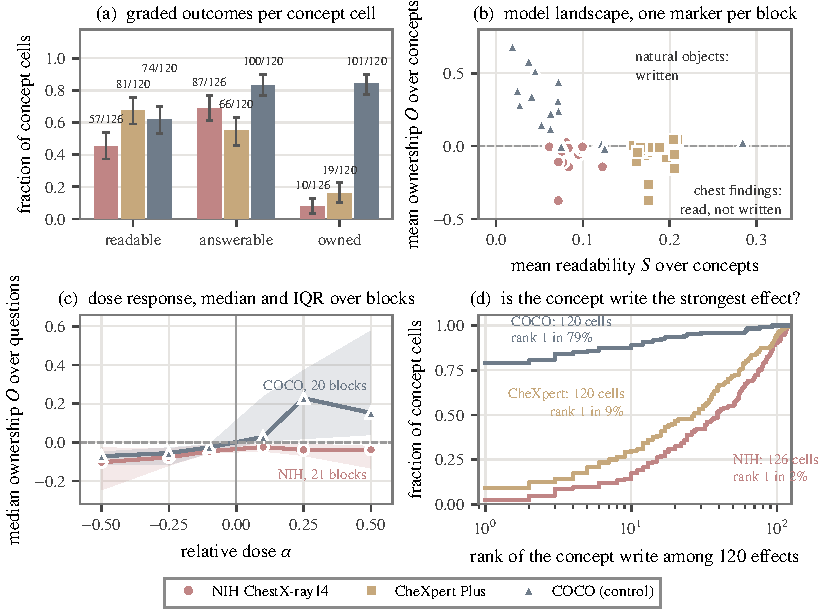
\includegraphics[width=\textwidth]{figures/fig2_overview.pdf}
    \caption{\textbf{Reading, answering, and writing across the grid.} (a) Readable, answerable, and owned cells per dataset (counts on the bars; descriptive bootstrap intervals over cells). (b) Mean readability against mean ownership per checkpoint. (c) Median ownership against the relative dose (median and interquartile band across the \cfDoseBlocksNih{} NIH and \cfDoseBlocksCoco{} COCO blocks with the dose module). (d) Rank of the concept write among the 120 compared effects.}
    \label{fig:overview}
\end{figure}

\subsection{The seed finding replicates on new patients}
\label{sec:seed}

We build on a two-model NIH study of Qwen2.5-VL-7B and LLaVA-1.5-7B (Appendix~\ref{app:seed}). In a 600-image cohort disjoint from every earlier cohort, we reproduce its central result (Table~\ref{tab:cf-seed}). The Effusion write raises the Effusion answer by $\cfSeedWEff$. This increase exceeds the random 95th percentile ($\cfSeedEffRandP$) and sham ($\cfSeedEffSham$). It ranks second among the 120 compared effects. Yet the Nodule direction raises the Effusion answer by $\cfSeedWNodule$. Effusion ownership is $O_{\mathrm{Effusion}}=\cfSeedEffO$ (95\% CI $[\cfSeedEffOLo,\cfSeedEffOHi]$), matching the original $-0.057$ $[-0.069,-0.045]$. We also reproduce the prompt dependence of Mass. Effusion and Cardiomegaly are the most readable chest concepts, with mean selectivity $\cfSelEffusion$ and $\cfSelCardiomegaly$ over \cfChestProbeBlocks{} chest blocks. Effusion is owned in \cfEffusionOwnedBlocks{} of \cfChestBlocks{} chest blocks. In \cfEffusionOwnedSmall{} of these blocks, $O_{\mathrm{Effusion}}\leq0.03$.

\subsection{The attribution deficit across the grid}
\label{sec:deficit}

On the chest sets, ownership is the rarest and least stable of the three grades. An effect floor of $0.05$ on both $W_{q,q}$ and $O_q$ retains \cfChestFloored{} of the \cfChestOwned{} owned chest cells (\cfChestFlooredPct\% of \cfChestAnswerableN{}), compared with \cfCocoFloored{} of the \cfCocoOwned{} owned COCO cells (\cfCocoFlooredPct\%). Ownership survives both probe refits on resampled patients in \cfRefitGradeStableNih{} of the \cfRefitGradeOwnedNih{} owned NIH cells, compared with \cfRefitGradeStableCoco{} of \cfRefitGradeOwnedCoco{} on COCO (Table~\ref{tab:cf-refit}). Clinical writes are not selective on the chest sets. To compute the write-flow share, we take the positive part of every entry of $W$ and average over checkpoints. We then divide the sum of the six own-question entries by the total. The written concept's own question receives \cfOwnShareNih\% of the positive answer change on NIH and \cfOwnShareChex\% on CheXpert, compared with \cfOwnShareCoco\% on COCO (Figure~\ref{fig:cf-w-structure}). This pattern is the attribution deficit. The model makes the concept readable to a probe. The probe's direction is not a handle on the concept. Writing it back moves other findings' answers as much as the concept's own.

Figure~\ref{fig:example} shows this pattern in individual images. On a chest radiograph, the Effusion and Nodule writes raise the same answers. The competing write raises the Effusion answer more than the Effusion write does. On a natural image, the dog write moves only the dog answer. The write matrix reveals two components of the deficit (Figure~\ref{fig:write-matrices}, Table~\ref{tab:cf-controls}). First, concept writes in the chest datasets have little effect on their own answers. The median $W_{q,q}$ is $\cfMedianWqqNih$ on NIH and $\cfMedianWqqChex$ on CheXpert, compared with $\cfMedianWqqCoco$ on COCO. Second, competing directions share the effect whenever a chest write moves an answer (Table~\ref{tab:cf-contingency}). Across the grid, the Atelectasis, Effusion, and Consolidation directions raise each other's answers by similar amounts. On COCO, the diagonal entry of $W$ dominates its row. On NIH and CheXpert, the row is flat or peaks off the diagonal. At every Qwen2.5-VL size, a competing direction raises the Effusion answer more than the Effusion direction does: Cardiomegaly at 3B, Nodule at 7B and 32B, and Atelectasis at 72B.

\subsection{The write mechanism is intact on natural objects}
\label{sec:coco}

On COCO, the same procedure yields the opposite result (Table~\ref{tab:cf-main}, right block). Object ownership holds in \cfCocoOwned{} of \cfCocoOwnedN{} cells (\cfCocoOwnedPct\%). Ownership margins span $\cfCocoMarginMin$--$\cfCocoMarginMax$ in the Qwen, Lingshu, and Gemma families. \cfCocoRefMet{} cells meet the steering reference. Only \cfCocoCompetitor{} cells have a stronger competitor. \cfCocoBlocksFourPlus{} of the \cfCocoBlocks{} checkpoints with a COCO block own at least four of the six objects. Dose response tracks the write. On COCO, median ownership across questions and blocks rises from $\cfDoseCocoLow$ at $\alpha=-0.1$ to $\cfDoseCocoPeak$ at $\alpha=+0.25$. Median ownership remains positive at $\alpha=+0.5$ ($\cfDoseCocoHalf$). On NIH, median ownership stays between $\cfDoseNihMin$ and $\cfDoseNihMax$ at every dose (Figure~\ref{fig:overview}c). The write, direction construction, reference family, and decision rules thus work as intended.

Task difficulty does not explain the contrast. Six small or fine-grained COCO categories---handbag, book, backpack, traffic light, knife, and cell phone---chosen by a rule fixed before the grid was built are fitted, written and graded exactly like the six easy objects in the same blocks and rows. They are owned in \cfFgFineOwned{} of \cfFgFineCells{} cells, a rate of \cfFgFineRate{} against \cfFgEasyRate{} for the easy six (\cfFgEasyOwned{} of \cfFgEasyCells{}). Median clean-answer AUROC is \cfFgFineAuroc{} against \cfFgEasyAuroc{}. Median probe selectivity is \cfFgFineSel{} against \cfFgEasySel{} (Table~\ref{tab:cf-fgobj}). Object size and fine-grainedness do not reduce ownership. Matching chest cells to natural-image cells of comparable difficulty preserves the contrast. We pair each chest cell with every natural-image cell whose matching variables lie within \cfFgWindow{} of the chest cell's values. We calculate ownership rates over the surviving pairs. Matching on probe selectivity alone pairs all \cfFgMatchSelN{} of \cfFgMatchSelCells{} chest cells and leaves ownership rates at \cfFgMatchSelChest{} against \cfFgMatchSelNat{} (difference $\cfFgMatchSelDiff$, 95\% interval $[\cfFgMatchSelLo,\cfFgMatchSelHi]$ over a cluster bootstrap whose unit is the model). Matching on clean-answer AUROC alone pairs \cfFgMatchAnsN{} and leaves \cfFgMatchAnsChest{} against \cfFgMatchAnsNat{}. Matching on both pairs \cfFgMatchBothN{} and leaves \cfFgMatchBothChest{} against \cfFgMatchBothNat{}. Probe quality does not separate the two sides: every chest cell finds a natural-image partner at its own selectivity, and ownership rates remain unchanged. Answer accuracy is the axis that excludes chest cells from the comparison. The chest cells that survive this matching already have accurate clean answers. The deficit is specific to clinical concepts rather than to task difficulty.

\begin{figure}[t]
    \centering
    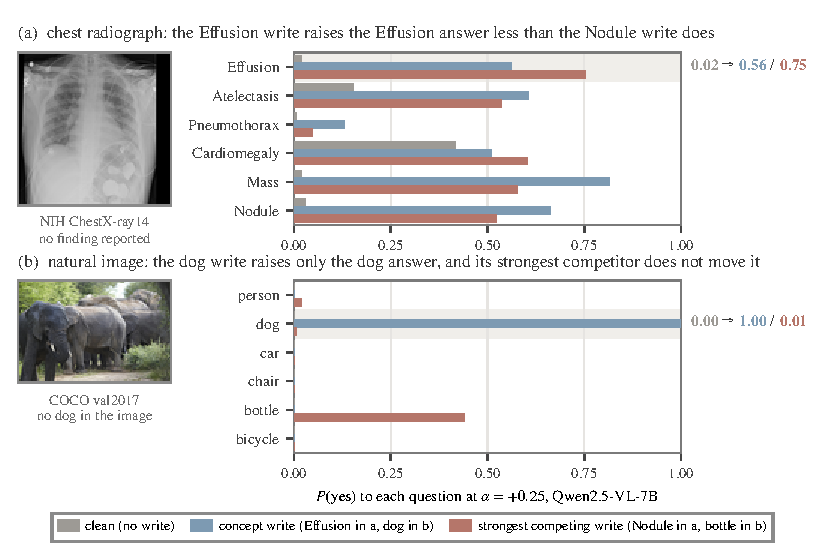
\includegraphics[width=\textwidth]{figures/fig3_example.pdf}
    \caption{\textbf{Two images, six questions, three writes.} $P(\mathrm{yes})$ per question for one NIH radiograph (top) and one COCO image (bottom) under the clean input, the concept write, and the strongest competing write, at $\alpha=+0.25$ in Qwen2.5-VL-7B. The Effusion write raises the Effusion answer from $0.02$ to $0.56$ and the Nodule write to $0.75$; the dog write moves the dog answer from $0.00$ to $1.00$ and nothing else.}
    \label{fig:example}
\end{figure}

\begin{figure}[t]
    \centering
    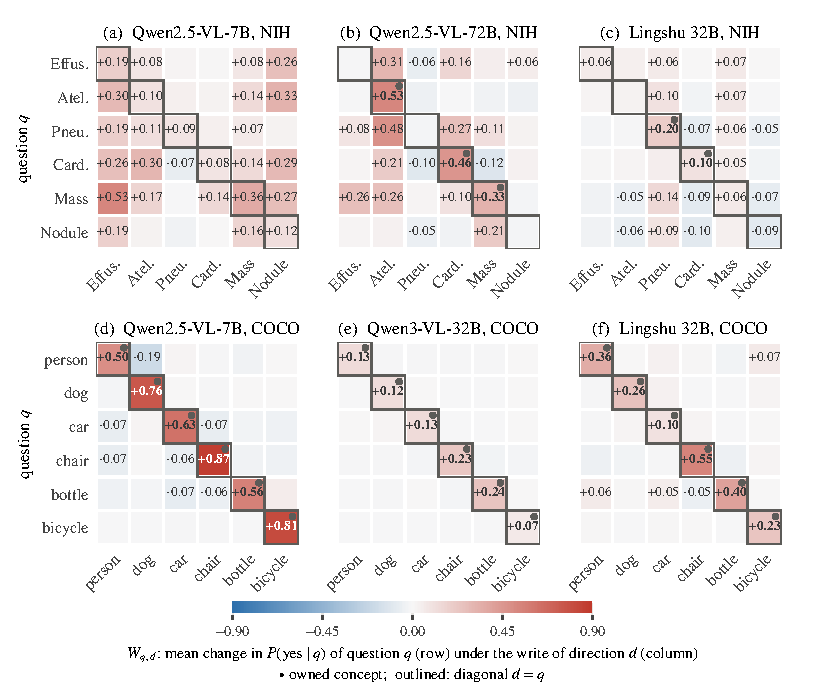
\includegraphics[width=\textwidth]{figures/fig4_write_matrices.pdf}
    \caption{\textbf{Write matrices.} $W_{q,d}$, the mean change in $P(\mathrm{yes})$ of question $q$ (rows) under the write of direction $d$ (columns), for three checkpoints on NIH (top) and three on COCO (bottom); the diagonal is outlined and owned concepts carry a dot. On COCO the diagonal dominates its row; on NIH the rows are flat or peak off the diagonal.}
    \label{fig:write-matrices}
\end{figure}

\subsection{Ownership belongs to the representation and the reader together}
\label{sec:reader}

Gemma~3 shares one SigLIP tower across its 4B, 12B, and 27B checkpoints. MedGemma shares one MedSigLIP tower across 4B and 27B. LLaVA-1.5 shares one CLIP tower across 7B and 13B. We intervene primarily at the tower's final block. This design changes the reader while holding the representation and write fixed. Within each family, pooled features, fitted probes, and lifted write vectors are identical across sizes. The connector and language model that read them differ. Features and write vectors are bit-identical for Gemma~3 4B and 12B and for LLaVA-1.5, and equal within one bf16 rounding step for Gemma~3 27B and MedGemma 27B. Raw model-space cosines between corresponding write vectors exceed $\cfPairsTowerCosMin$ for every concept and pair. Readability is identical across sizes by construction. The connector and language model produce every difference in Figure~\ref{fig:readers} by reading the same written representation differently. The median paired difference is \cfPairsRatioMin{}--\cfPairsRatioMax{} times the refit standard deviation. It exceeds that standard deviation in \cfPairsRatioAboveOne{} of the \cfPairsRatioN{} pairs with a refit estimate (Table~\ref{tab:cf-pairs}). On NIH Effusion, the identical write on the same 600 patients yields an $O_q$ difference of $\cfPairDeltaEffFourTwelve$ $[\cfPairDeltaEffFourTwelveLo,\cfPairDeltaEffFourTwelveHi]$ between Gemma~3 4B and 12B. The difference between 12B and 27B is $\cfPairDeltaEffTwelveTwentySeven$ $[\cfPairDeltaEffTwelveTwentySevenLo,\cfPairDeltaEffTwelveTwentySevenHi]$. In \cfPairsFiveOrSix{} of the \cfPairsN{} shared-tower pair--dataset combinations, the paired patient-bootstrap interval for $\Delta O_q$ excludes zero for five or six of the six concepts. The median $|\Delta O_q|$ is \cfPairsRatioMin{}--\cfPairsRatioMax{} times the families' refit standard deviation (up to \cfPairsRatioSingleMax{} times for single concepts). In 12B, competing directions own the chest answers outright ($O_{\mathrm{Effusion}}=\cfOGemmaTwelveEff$ on both chest sets, $O_{\mathrm{Mass}}=\cfOGemmaTwelveMass$, $O_{\mathrm{Pneumothorax}}=\cfOGemmaTwelvePneu$). In 27B, no direction moves these answers ($\cfOGemmaTwentySevenEff$, $\cfOGemmaTwentySevenMass$, $\cfOGemmaTwentySevenPneu$). In 4B, the clean answer is yes on \cfGemmaFourYesMin--\cfGemmaFourYesMax\% of chest rows. Every own write lowers its answer's logit margin by more than any competing write raises it ($O^m_q$ from $\cfPairsGemmaFourOmNear$ to $\cfPairsGemmaFourOmFar$, all intervals below zero). MedGemma 4B and 27B differ in the same way (Pneumothorax $\cfOMedFourPneu$ versus $\cfOMedTwentySevenPneu$ and Edema $\cfOMedFourEdema$ versus $\cfOMedTwentySevenEdema$ on CheXpert). LLaVA-1.5 7B and 13B own no concepts on either chest set, yet own \cfLlavaSevenCoco{} and \cfLlavaThirteenCoco{} COCO objects with the same write. The chest cells these readers own (Gemma~3 12B: Nodule on NIH, Edema on CheXpert; MedGemma 4B: Cardiomegaly and Edema on CheXpert) carry the least evidential weight. The reader effect spans the whole matrix, regardless of which cell crosses zero.

This design forms the reader half of a crossing. The other half replaces the representation. We load one checkpoint's vision tower behind the other's connector and language model. Of the host tower's \cfSwapTowerTensors{} tensors, \cfSwapTensors{} carry weights. We replace every one and verify bitwise equality with the donor's (\cfSwapParamsM{} million parameters). None of the \cfSwapOutside{} tensors outside the tower changes. Gemma~3 4B and MedGemma 4B give \cfSwapCombos{} combinations of tower and reader on each dataset. We grade each combination on the same \cfSwapRows{} rows at the same dose against the same references. Written directions travel with the tower that produced them (Table~\ref{tab:cf-towerswap}). On NIH and CheXpert, no combination owns a finding: \cfSwapChestOwned{} of \cfSwapChestCells{} cells across the \cfSwapChestCombos{} combinations. On COCO, the same crossing owns \cfSwapCocoOwned{} of \cfSwapCocoCells{} cells. Each native combination owns \cfSwapCocoNativeMin{} of the six objects. The Gemma tower behind the MedGemma reader owns \cfSwapCocoGemmaTowerCross{}. The MedGemma tower behind the Gemma reader owns \cfSwapCocoMedTowerCross{}. Replacing the representation alone and replacing the reader alone each leave every clinical concept unwritable. Natural-image concepts remain writable under three of the four combinations. Ownership is a property of the representation and the reader together.

The crossover measures each factor's effect with the other held fixed. On NIH, the mean absolute reader effects on the six own-question write magnitudes are \cfSwapReaderNihMin{} and \cfSwapReaderNihMax{} in the two crossovers, against a tower effect of \cfSwapTowerNihMin{} in both. On CheXpert, the reader and tower effects are \cfSwapReaderChexMin{} and \cfSwapTowerChexMin{}, respectively. On COCO, the tower effect is larger: \cfSwapTowerCocoMin{} against \cfSwapReaderCocoMin{}. Neither factor dominates on the chest sets. The crossover costs resolution rather than agreement. Across the \cfSwapNativeCells{} cells of the six native arms, the ownership contrast moves by at most \cfSwapNativeMaxDO{} from the published grade. On the crossover's smaller cohort, \cfSwapNativeUnresolved{} of the \cfSwapNativeOwnedFull{} published owned cells become unresolved.

Two readers of a shared-tower pair receive inputs that agree up to bf16 rounding. Replaying the consumed block's stored token tensors makes their inputs identical bit for bit (Table~\ref{tab:cf-replay}). A reader replaying its own block's tensors controls for the machinery. Across the \cfReplaySelf{} such replays, no verdict or ownership changes. Of these, \cfReplaySelfExact{} reproduce the block's own grade exactly; the third differs by at most $\cfReplayMaxDWSelf$ in a write magnitude. Across all \cfReplayBlocks{} replays, the largest change in a write magnitude is $\cfReplayMaxDW$. In total, \cfReplayMoved{} of \cfReplayCells{} concept cells move at all, and \cfReplayVerdictChanges{} verdicts and \cfReplayOwnedChanges{} ownership grades change. In \cfReplayDriftZero{} of the \cfReplayBlocks{} replays, the reader's own tower output already matches the stored tensor bit for bit. The exception is LLaVA-Med, whose fine-tuned tower departs from the stored tensor by up to \cfReplayDriftMax{} against a mean absolute tensor entry of \cfReplayTensorMin{}--\cfReplayTensorMax{}. The cross-reader replays settle the rounding question. Across the \cfReplayPairs{} reader pairs, the mean absolute difference between the readers' own-question write magnitudes is \cfReplayPairOwnMin{}--\cfReplayPairOwnMax{} when each reader runs its own tower. Feeding both readers the same tensors changes that difference by at most \cfReplayChangeMax{}, or \cfReplayRelMax\% of its size. Input rounding does not explain what separates two readers of one tower.

\begin{figure}[t]
    \centering
    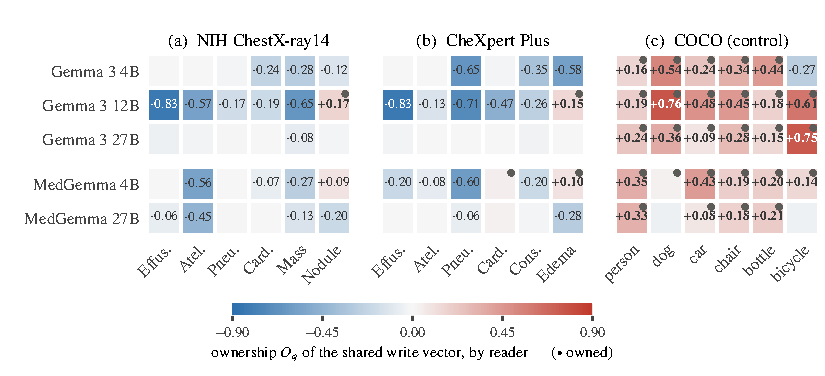
\includegraphics[width=\textwidth]{figures/fig5_same_write.pdf}
    \caption{\textbf{Same write, different reader.} Ownership $O_q$ per concept on NIH, CheXpert, and COCO for Gemma~3 4B/12B/27B and MedGemma 4B/27B, whose probes and write vectors are identical across sizes within each family; dots mark owned cells and hatching marks ceiling cells (clean answer beyond $0.99$ or $0.01$ on more than 90\% of rows).}
    \label{fig:readers}
\end{figure}

\subsection{The direction the reader responds to}
\label{sec:ansdir}

The same representation contains the reader's handle. For each question, we use ridge regression to fit the model's own clean answer margin from the same projected, train-scaled features, using the first 3{,}000 rows of the training cohort in fixed manifest order. This order is a seeded shuffle on NIH and a hash of patient or image identity on CheXpert and COCO; neither labels nor answers enter it. We select each question's penalty by five-fold cross-validated $R^2$ over $\{0.1,1,10,100\}$. Across the \cfAnsAlphaCells{} fitted questions, the selected penalty is $1$ for \cfAnsAlphaOne{}, $10$ for \cfAnsAlphaTen{}, and $100$ for \cfAnsAlphaHundred{}. Cross-validation splits rows. On CheXpert and COCO, each of the 3{,}000 rows represents a distinct patient or image. On NIH, the rows come from \cfAnsTrainUnitsNih{} patients. We lift the fitted direction as we lift a probe normal and write it at the same dose against the same reference family (Table~\ref{tab:cf-ansdir}). This answer direction $a_q$ is a handle where the label direction is not. Across the \cfAnsChestN{} chest cells in the \cfAnsChestBlocks{} scored chest blocks (Table~\ref{tab:cf-ansdir}, top), $a_q$ is owned in \cfAnsChestOwnedA{} and the label direction in \cfAnsChestOwnedLabel{}. The answer direction's write beats the strongest logistic competitor in \cfAnsChestBeats{}. Across the five held-out templates, $a_q$ remains owned in \cfAnsdirtChestKept{} of \cfAnsdirtChestKeptN{} chest and \cfAnsdirtCocoKept{} of \cfAnsdirtCocoKeptN{} COCO (cell, template) pairs (Table~\ref{tab:cf-ansdir}, bottom). Across all pairs, regardless of cell ownership under the primary template, $a_q$ is owned in \cfAnsdirtChestOwnedPairs{} of \cfAnsdirtChestPairsAll{} chest and \cfAnsdirtCocoOwnedPairs{} of \cfAnsdirtCocoPairsAll{} COCO (cell, template) pairs. In Qwen2.5-VL-7B, it is owned for \cfAnsQwenOwnedNih{} of six NIH concepts (Effusion $O^a=\cfAnsQwenEffO$ with an own write of $\cfAnsQwenEffW$) and all \cfAnsQwenOwnedChex{} CheXpert concepts. In Lingshu 32B, it is owned for \cfAnsLingOwnedNih{} NIH and \cfAnsLingOwnedChex{} CheXpert concepts. In Gemma~3 12B, it is owned for \cfAnsGemOwnedNih{} NIH and \cfAnsGemOwnedChex{} CheXpert concepts. We summarise the raw model-space cosine between the answer direction and the probe normal by the median over each block's six concepts. These medians span $\cfAnsCosQwenMin$--$\cfAnsCosQwenMax$ across the two chest blocks of Qwen2.5-VL-7B and $\cfAnsCosLingMin$--$\cfAnsCosLingMax$ across those of Lingshu 32B, compared with $\cfAnsCosCocoMin$--$\cfAnsCosCocoMax$ across the COCO blocks. The cosine whitened by the training-feature covariance in the projected, train-scaled space has a median over each dataset's cells of $\cfValCosSigmaChestMin$--$\cfValCosSigmaChestMax$ on the two chest sets and $\cfValCosSigmaCoco$ on COCO. The metrics differ most on the CheXpert block of Lingshu 32B, where the median over its six concepts is $\cfValCosRawLingChex$ raw and $\cfValCosSigmaLingChex$ whitened. The answer direction reads the model, not the label. Over the \cfValAurocAnsChestN{} chest cells, its median AUROC against the report label is $\cfValAurocAnsChest$, compared with $\cfValAurocProbeChest$ for the probe. Against the model's own clean answer, its median AUROC is $\cfValAurocAnsCleanChest$, compared with $\cfValAurocProbeCleanChest$ for the probe (median over the \cfValAurocAnsCleanChestN{} chest cells whose clean answers take both values; Table~\ref{tab:cf-validation}). In Qwen2.5-VL-7B on NIH, the label AUROC is $\cfValAurocAnsQwenNih$ for the answer direction and $\cfValAurocProbeQwenNih$ for the probe. The clean-answer AUROC is $\cfValAurocAnsCleanQwenNih$ and $\cfValAurocProbeCleanQwenNih$, respectively. Ownership compares the six directions of one construction within each question's row of $W$. The column-selectivity index $S_d=W_{d,d}/\sum_q|W_{q,d}|$ of Section~\ref{sec:robust-geometry} measures the share of a direction's effect that lands on its own question. Across the \cfAnsColSelChestN{} chest cells, the median $S_d$ is $\cfAnsColSelChest$ for answer directions and $\cfAnsColSelLabelChest$ for label directions in the same blocks. The corresponding medians are $\cfAnsColSelCoco$ and $\cfAnsColSelLabelCoco$ over the \cfAnsColSelCocoN{} COCO cells. On the chest sets, both answer and label directions move the other five answers along with their own. The row comparison separates them: the answer direction wins in \cfAnsChestOwnedA{} of \cfAnsChestN{} cells against \cfAnsChestOwnedLabel{} for the label direction. On natural images, the readable and writable directions coincide. On chest radiographs, the model answers along a direction the probe does not read.

We test writes from both families at four endpoints used to fit neither direction: the negated form of the concept's yes/no question, a two-alternative forced choice against the concept's strongest competitor in each of the two presentation orders, and the finding word's log-probability in a report continuation (Table~\ref{tab:cf-semend}). Across the \cfSemCells{} endpoint cells of the \cfSemBlocks{} scored blocks, the label direction is owned in \cfSemLabelOwned{} and the answer direction in \cfSemAnswerOwned{}. The negated question moves opposite to the affirmative one in \cfSemNegOpposite{} of the \cfSemNegN{} concept--block pairs. The forced choice is owned in both presentation orders in \cfSemForcedOwned{} of \cfSemForcedN{} pairs, with a mean absolute gap of \cfSemGapMin{}--\cfSemGapMax{} between orders. The report continuation is owned in \cfSemReportOwned{} of \cfSemReportCells{} cells. The separation between the two families persists across endpoints.

Ownership predicts endpoint effects beyond write magnitude, probe selectivity, and clean-answer AUROC. Regressing each endpoint effect on these three quantities with endpoint dummies gives a base $R^2$ of \cfSemIVBaseMin{}--\cfSemIVBaseMax{}. Adding the ownership contrast raises it by \cfSemIVMin{}--\cfSemIVMax{}. The added-variance interval excludes zero in all \cfSemIVExcl{} of the \cfSemIVN{} block-and-family combinations. Ownership is a predictive criterion, not a label.

\subsection{Size and family}
\label{sec:families}

Ownership on the chest sets is concentrated among a few readers and varies by concept and dataset (Figure~\ref{fig:ladders}; Table~\ref{tab:cf-models}). Qwen2.5-VL owns no concepts at 3B or 7B. At 32B, it owns Cardiomegaly. At 72B, it owns Atelectasis ($O=\cfOQwenSeventyTwoAtel$), Cardiomegaly, and Mass. Effusion is anti-owned at every size. Lingshu, the medical Qwen2.5-VL derivative, owns three CheXpert concepts at 7B. At 32B, it owns five, the highest clinical ownership in the grid. InternVL3.5 answers every NIH question at every size. On the chest sets, its writes remain within $\cfInternvlWqqMax$ of zero. LLaVA-1.5 reads the chest concepts. It answers none above chance. It owns none.

\subsection{Controls and alternatives}
\label{sec:controls}

The reference family and additional controls behave as designed across the grid (Figure~\ref{fig:overview}d; Table~\ref{tab:cf-controls}). Owned concept writes rank 1--6 among the 120 compared effects. The concept write typically ranks in the top decile on the chest sets.

\label{sec:robust-geometry}

\paragraph{Geometry, scale, saturation, refits, numerics.} No measurement alternative explains the deficit (Tables~\ref{tab:cf-geometry}--\ref{tab:cf-validation}; Appendix~\ref{app:cf-robustness}). The strongest competitor matches the most similar direction or the most co-occurring label at chance rate. Logit-scale verdicts agree in \cfScaleAgree{} of \cfScaleAgreeN{} cells. COCO blocks are more saturated than chest blocks. Restricting each cell to unsaturated rows preserves the full owned grade in \cfScaleUnsatGradeKept{} of \cfScaleUnsatGradeN{} owned chest cells. We recompute the steering reference on those rows. We evaluate the simultaneous max-$T$ advantage over the same six-direction family. Refits change $O_q$ by a median of \cfScaleRefitMedian{}. The column-selectivity index $S_d=W_{d,d}/\sum_q|W_{q,d}|$ divides a direction's signed effect on its own question by its summed absolute effect on the six questions. Across cells, its median is \cfValColSelNih{} on NIH and \cfValColSelChex{} on CheXpert, versus \cfValColSelCoco{} on COCO (Table~\ref{tab:cf-validation}). $S_d$ retains negative effects and weights every cell equally. It therefore differs from the write-flow share of Section~\ref{sec:deficit}, which retains only positive effects and pools them over checkpoints. On CheXpert, restricting evaluation to rows with a known label preserves the sign of $O_q$ in \cfValKnownSignAgree{} of \cfValKnownN{} cells. Re-grading the same fitted directions on \cfValidRows{} CheXpert films labelled by radiologist consensus reproduces the owned grade in \cfValidOwnedAgree{} of \cfValidCells{} cells (Table~\ref{tab:cf-valid}). These films share no patient with any campaign cohort. Both grades use directions fitted on report-derived labels. Refitting the six directions on the radiologist labels themselves changes the fit's label source. Across the \cfValidfitBlocks{} CheXpert blocks with this refit, the expert-label and report-label directions have a median raw model-space cosine of \cfValidfitCosRaw{} and a median whitened cosine of \cfValidfitCosWhitened{}. The expert-label refit reads the radiologist labels with a median cross-fitted AUROC of \cfValidfitAurocExpert{}, versus \cfValidfitAurocReportDir{} for the report-label direction on the same films. Written on the test rows under the same references, the expert-label directions are owned in \cfValidfitOwnedExpert{} of \cfValidfitCells{} cells, the report-label directions in \cfValidfitOwnedReport{} (Appendix~\ref{app:cf-robustness}). Rescoring in fp32 and at batch size one changes $W$ by at most \cfPrecisionMaxDW{} and alters \cfPrecisionGradeChanges{} of \cfPrecisionGradeCells{} grades (Table~\ref{tab:cf-precision}).

\paragraph{Alternative direction constructions.} The deficit persists beyond the logistic normal. We test four alternative directions with the same projected, train-scaled features and write protocol (Table~\ref{tab:cf-altdir}): the difference of class means, the Haufe pattern $\Sigma\boldsymbol\beta_c$ \citep{haufe2014interpretation}, the normal orthogonalised against the other five normals, and the normal refitted on features residualised against the other five labels. Across the \cfAltdirBlocks{} scored blocks (\cfAltdirBlocksPerDs{} per dataset), each construction owns \cfAltdirChestPctMin{}--\cfAltdirChestPctMax\% of chest cells and \cfAltdirCocoPctMin{}--\cfAltdirCocoPctMax\% of COCO cells. For the difference-of-means and pattern directions, we measure the absolute raw model-space cosine with the logistic normal. The median over the six concepts in each block ranges from $\cfAltdirCosMin$ to $\cfAltdirCosMax$. Each of these two directions owns more NIH cells and fewer COCO cells than the logistic normal. Lifted as displacements, they respectively own \cfAltdirdChestDom{} and \cfAltdirdChestPattern{} of \cfAltdirdChestN{} chest cells and \cfAltdirdCocoDom{} and \cfAltdirdCocoPattern{} of \cfAltdirdCocoN{} COCO cells (Table~\ref{tab:cf-altdir}). Every construction preserves the chest-to-COCO gap. At least one construction owns \cfAltdirNihAny{} of \cfAltdirNihN{} cells on NIH and \cfAltdirChexAny{} of \cfAltdirChexN{} on CheXpert, compared with \cfAltdirCocoAny{} of \cfAltdirCocoN{} on COCO. Extending the clinical family to every additional dataset label with enough support retains \cfExtcompRetained{} of the \cfExtcompOwned{} owned cells in the \cfExtcompBlocks{} scored blocks (Table~\ref{tab:cf-altdir}). We combine projection, sex, age, and the findings into one nine-direction family. The three attributes are non-clinical properties of the same radiographs. Their probes read them at least as well as the clinical probes read the findings. Median probe AUROC per attribute is \cfAttrAurocMin{}--\cfAttrAurocMax{}, compared with \cfAttrClinAuroc{} for findings in the same blocks. All \cfAttrReadable{} of \cfAttrChestAttrN{} attribute cells are readable. Both kinds of question carry the same steering reference in all \cfAttrRefBlocks{} blocks. Attributes own \cfAttrAllAttrOwned{} of \cfAttrAllAttrN{} cells; findings own \cfAttrAllClinOwned{} of \cfAttrAllClinN{}, the same rate. Among cells whose clean answer meets the answer-capable rule, attributes own \cfAttrCapAttrOwned{} of \cfAttrCapAttrN{} and findings \cfAttrCapClinOwned{} of \cfAttrCapClinN{}. Pairing each attribute cell with clinical cells from its own block within \cfAttrPairWindow{} clean-answer AUROC yields \cfAttrPairAttrN{} pairs, with attributes owned in \cfAttrPairAttrOwned{} and findings in \cfAttrPairClinOwned{}. The within-image comparison shows that a non-clinical property of the same film is no more writable than a finding. Each attribute question uses one of \cfAttrqPhrasings{} phrasings scored on the calibration rows. The written phrasing reaches a median clean-answer AUROC of \cfAttrqWrittenAuroc{} against \cfAttrqSelectedAuroc{} for the most answerable phrasing of the same cell. The median gap is \cfAttrqGain{} over the \cfAttrqCells{} attribute cells. On NIH, ownership is \cfAttrNihAttrOwned{}/\cfAttrNihAttrN{} for attributes and \cfAttrNihClinOwned{}/\cfAttrNihClinN{} for findings (Table~\ref{tab:cf-attr}). We weight writes along the logistic directions by the softmax of token probe scores or restrict them to the top quarter of tokens at four times the weight (twice the Frobenius norm of the uniform write). Across the \cfTokenwChestBlocks{} chest blocks with these writes, the softmax write owns \cfTokenwSoftChestOwned{} of \cfTokenwChestCells{} cells, the top-quarter write owns \cfTokenwTopqChestOwned{}, and the uniform write owns \cfTokenwUniformChestOwned{}. On COCO, the softmax and top-quarter writes own \cfTokenwSoftCocoOwned{} and \cfTokenwTopqCocoOwned{} of \cfTokenwCocoCells{} cells (Table~\ref{tab:cf-altdir}). Concentrating the write where the probe reads does not create a clinical handle.


\FloatBarrier
